\documentclass[11pt,a4paper]{article}
\usepackage[utf8]{inputenc}
\usepackage[T1]{fontenc}
\usepackage[english]{babel}
\usepackage{amsmath,amssymb}
\usepackage{graphicx}
\usepackage{geometry}
\usepackage{hyperref}
\usepackage{booktabs}

\geometry{margin=2.2cm}

\title{\textbf{Clasificador bayesiano generativo\\para d\'igitos MNIST}}
\author{Probabilidad y Estad\'istica --- Proyecto final}
\date{}

\begin{document}
\maketitle

%-----------------------------------------------------------
\section{Problema}
%-----------------------------------------------------------

El problema consiste en asignar una clase
\[
  y \in \{0,1,2,\dots,9\}
\]
a una imagen
\[
  x \in \mathbb{R}^{784}
\]
(pues cada imagen es de $28\times 28$ p\'ixeles y $28\cdot 28 = 784$).

Para clasificar, asignamos un puntaje a cada clase y escogemos la clase con
mayor puntaje. Esa operaci\'on se representa con $\arg\max$:
\[
  \hat{y} = \arg\max_{c\in\{0,\dots,9\}} S_c(x).
\]

Como queremos un enfoque probabil\'istico, el puntaje m\'as natural es la
probabilidad posterior $P(y=c\mid x)$. Entonces:
\[
  \hat{y} = \arg\max_{c\in\{0,\dots,9\}} P(y=c\mid x).
\]

%-----------------------------------------------------------
\section{Metodolog\'ia}
%-----------------------------------------------------------

\subsection{El teorema de Bayes}

La cantidad $P(y=c\mid x)$ no se modela directamente. Usamos Bayes:
\[
  P(y=c\mid x) = \frac{P(y=c)\;p(x\mid y=c)}{p(x)}.
\]

Bayes cambia la pregunta: en vez de \emph{``dada la imagen, ?`qu\'e tan
probable es la clase?''}, pregunta \emph{``si yo supiera que la clase es $c$,
?`qu\'e tan compatible ser\'ia observar una imagen como $x$?''}.

Como $p(x)$ no depende de $c$:
\[
  \hat{y} = \arg\max_c P(y=c)\;p(x\mid y=c).
\]

Aplicando logaritmo:
\[
  \hat{y} = \arg\max_c \bigl[\log P(y=c) + \log p(x\mid y=c)\bigr].
\]

\subsection{Suposici\'on de modelado}

Suponemos que las im\'agenes de cada clase siguen una distribuci\'on normal
multivariada:
\[
  x\mid y=c \;\sim\; \mathcal{N}(\mu_c,\,\Sigma_c).
\]

No decimos que $y$ sigue una normal. La clase $y$ es discreta
($y\in\{0,1,\dots,9\}$). Lo que modelamos como normal es la imagen $x$
cuando ya sabemos la clase.

La densidad es:
\[
  p(x\mid y=c) = \frac{1}{(2\pi)^{d/2}\,|\Sigma_c|^{1/2}}\;
  \exp\!\Bigl(-\tfrac{1}{2}(x-\mu_c)^{\mathsf{T}}
  \Sigma_c^{-1}(x-\mu_c)\Bigr).
\]

\subsection{Estimaci\'on de m\'axima verosimilitud}

Los par\'ametros $\mu_c$ y $\Sigma_c$ se estiman desde los datos:

\[
  \hat{P}(y=c) = \frac{N_c}{N}, \qquad
  \hat{\mu}_c = \frac{1}{N_c}\sum_{i:\,y_i=c} x_i, \qquad
  \hat{\Sigma}_c = \frac{1}{N_c}\sum_{i:\,y_i=c}
    (x_i-\hat{\mu}_c)(x_i-\hat{\mu}_c)^{\mathsf{T}}.
\]

Regularizamos $\hat{\Sigma}_c$ a\~nadiendo $\varepsilon\,\mathbf{I}_d$ con
$\varepsilon=10^{-4}$ para garantizar invertibilidad.

\subsection{Regla de clasificaci\'on}

Sustituyendo la densidad normal y eliminando la constante
$\frac{d}{2}\log(2\pi)$:

\[
  \boxed{\;\hat{y} = \arg\max_c \Bigl[
    \log \hat{P}(y=c)
    - \tfrac{1}{2}\log|\hat{\Sigma}_c|
    - \tfrac{1}{2}(x-\hat{\mu}_c)^{\mathsf{T}}
      \hat{\Sigma}_c^{-1}(x-\hat{\mu}_c)
  \Bigr]\;}
\]

Cada t\'ermino tiene interpretaci\'on:
\begin{itemize}
  \item $\log \hat{P}(y=c)$: premia clases m\'as frecuentes.
  \item $-\frac{1}{2}\log|\hat{\Sigma}_c|$: penaliza clases con mucha
        dispersi\'on.
  \item $-\frac{1}{2}(x-\hat{\mu}_c)^{\mathsf{T}}\hat{\Sigma}_c^{-1}
         (x-\hat{\mu}_c)$: distancia de Mahalanobis entre la imagen y la
         media de la clase.
\end{itemize}

La Figura~\ref{fig:means} muestra las medias estimadas $\hat{\mu}_c$ de cada
clase, que representan el ``d\'igito promedio'' de cada clase.

\begin{figure}[htbp]
  \centering
  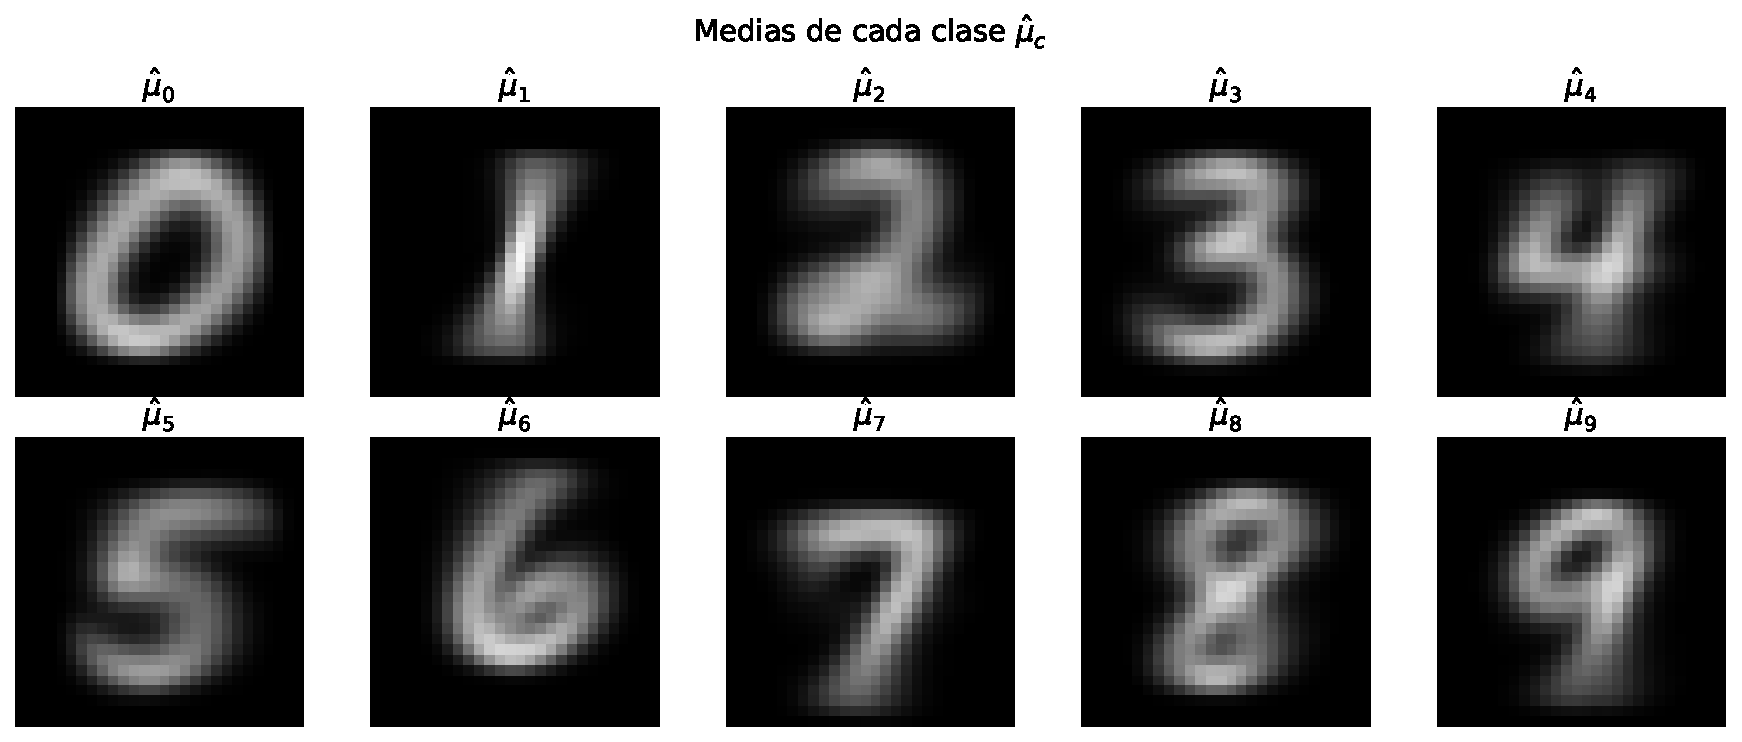
\includegraphics[width=\textwidth]{figs/means.pdf}
  \caption{Medias de cada clase $\hat{\mu}_c$ estimadas por m\'axima
           verosimilitud.}
  \label{fig:means}
\end{figure}

%-----------------------------------------------------------
\section{Resultados}
%-----------------------------------------------------------

El clasificador alcanza una exactitud global del
$86{,}55\,\%$ en el conjunto de prueba (10\,000 im\'agenes).

La Figura~\ref{fig:cov} muestra la varianza por p\'ixel de cada clase
(diagonal de $\hat{\Sigma}_c$), y la Figura~\ref{fig:confusion} presenta la
matriz de confusi\'on.

\begin{figure}[htbp]
  \centering
  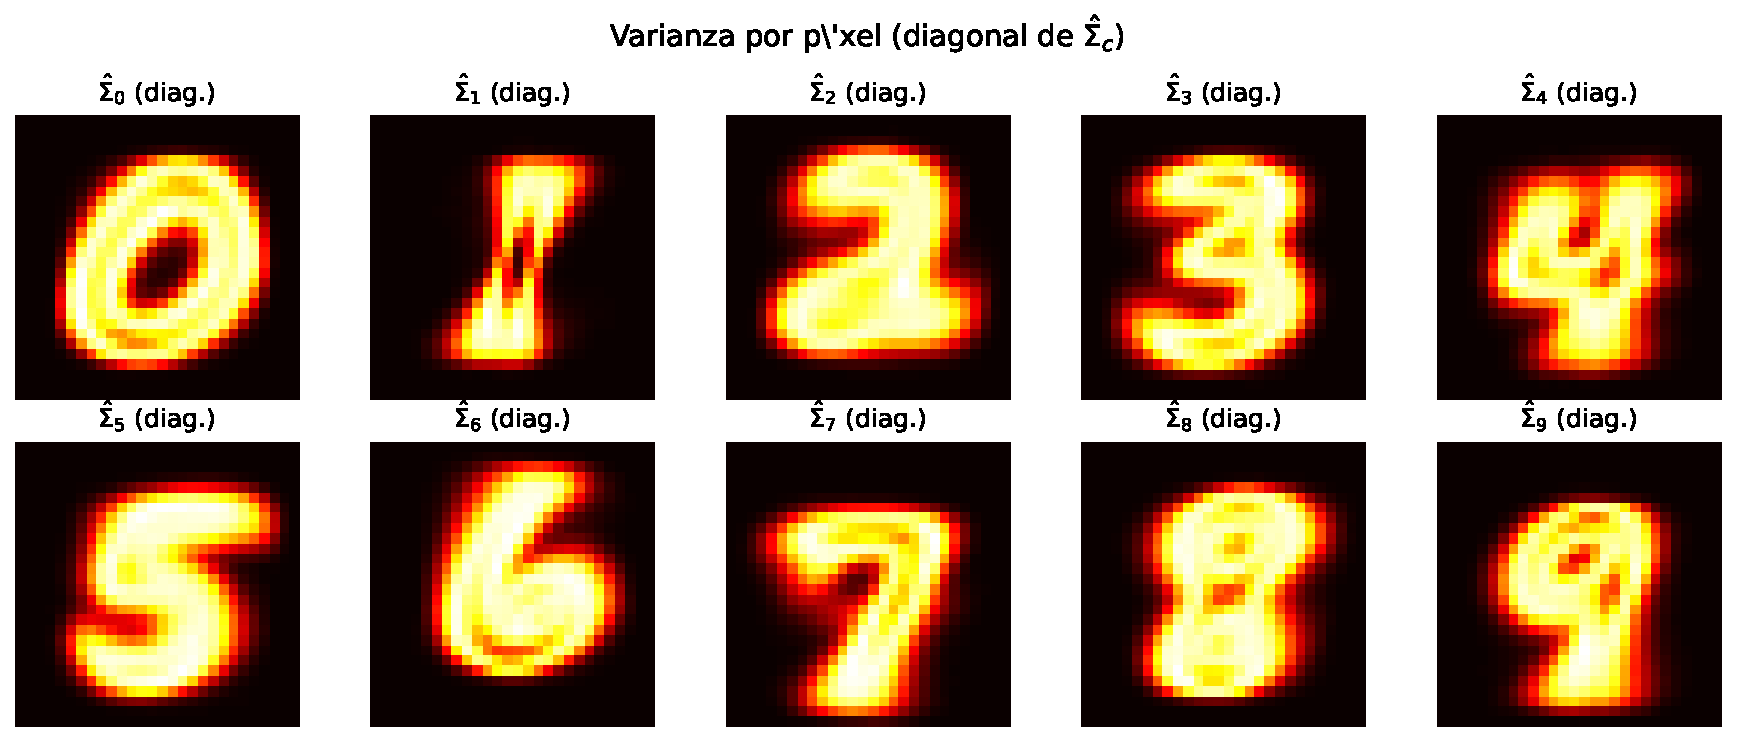
\includegraphics[width=\textwidth]{figs/cov_diag.pdf}
  \caption{Varianza por p\'ixel de cada clase (diagonal de
           $\hat{\Sigma}_c$). Las zonas m\'as brillantes indican mayor
           variabilidad.}
  \label{fig:cov}
\end{figure}

\begin{figure}[htbp]
  \centering
  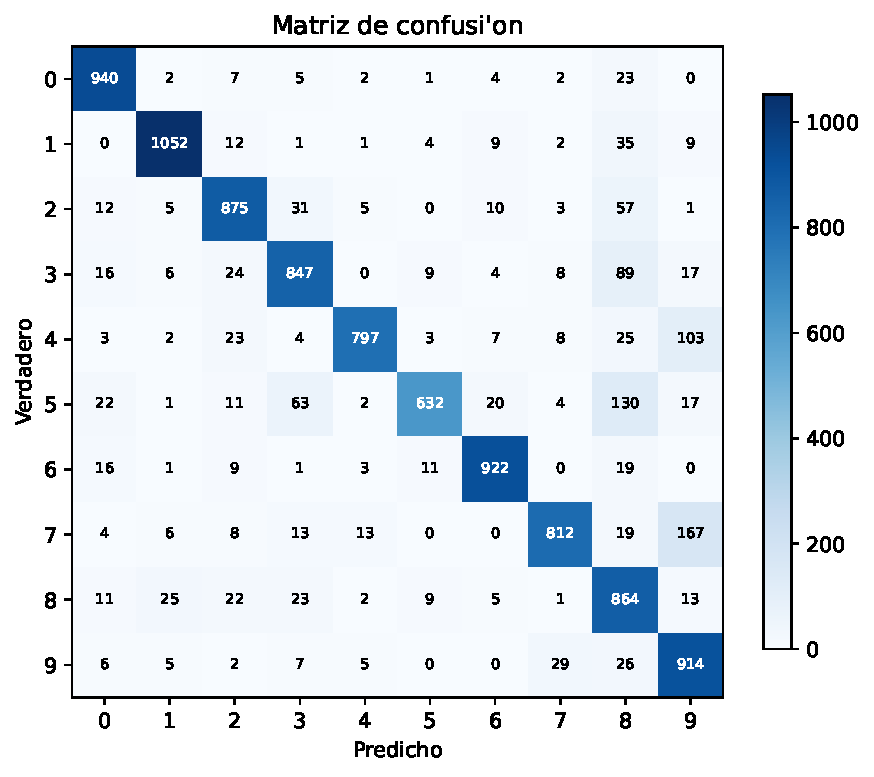
\includegraphics[width=0.75\textwidth]{figs/confusion.pdf}
  \caption{Matriz de confusi\'on del clasificador.}
  \label{fig:confusion}
\end{figure}

La exactitud por clase var\'ia significativamente (Figura~\ref{fig:acc}):
d\'igitos como el 0 y el 1 se clasifican con alta precisi\'on, mientras que
el 5 y el 7 presentan mayor tasa de error.

\begin{figure}[htbp]
  \centering
  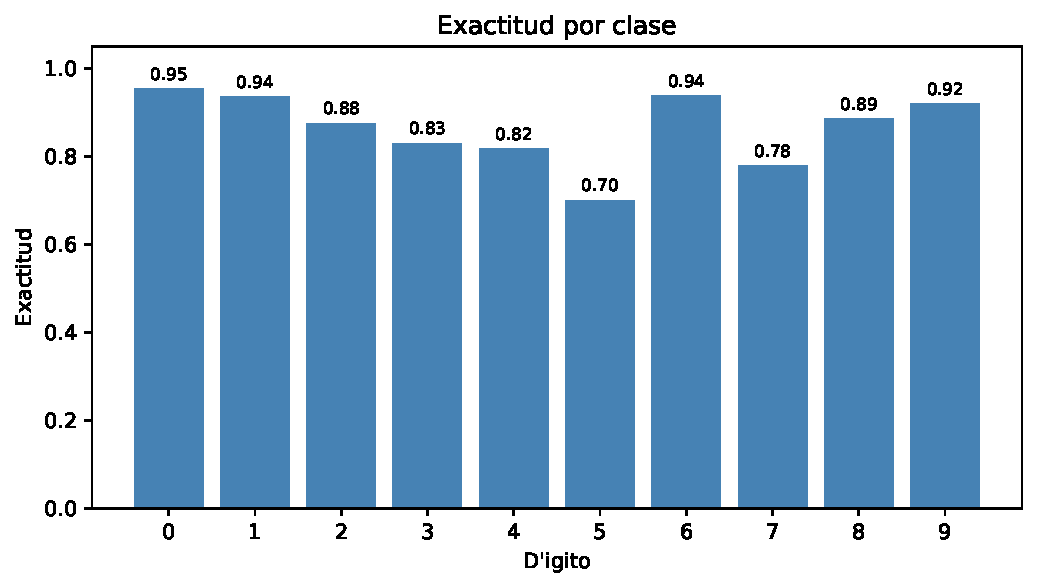
\includegraphics[width=0.85\textwidth]{figs/per_class_acc.pdf}
  \caption{Exactitud por clase.}
  \label{fig:acc}
\end{figure}

%-----------------------------------------------------------
\section{Conclusiones}
%-----------------------------------------------------------

Construimos un clasificador bayesiano generativo. Para cada clase $c$,
modelamos la distribuci\'on de las im\'agenes $x\mid y=c$ mediante una normal
multivariada. Estimamos los par\'ametros de cada clase con los datos de
entrenamiento por m\'axima verosimilitud y luego clasificamos una imagen nueva
escogiendo la clase que maximiza la probabilidad posterior $P(y=c\mid x)$.

La interfaz probabil\'istica permite cuantificar la \textbf{confianza} en cada
predicci\'on mediante las probabilidades posteriores normalizadas. La
confianza media es del $99{,}3\,\%$ y la mediana del $100{,}0\,\%$, lo que
indica que el modelo suele estar muy seguro de sus predicciones correctas;
sin embargo, los errores de clasificaci\'on tienden a ocurrir en casos con
confianza m\'as baja, lo cual es coherente con el marco probabil\'istico.

Como el denominador de Bayes no depende de la clase, la regla se reduce a
maximizar $\log p(x\mid y=c)+\log P(y=c)$, lo que hace la implementaci\'on
eficiente y sin necesidad de optimizaci\'on iterativa.

\end{document}
